\documentclass[10pt,a4paper]{report}
\usepackage[utf8]{inputenc}
\usepackage[german]{babel}
\usepackage[T1]{fontenc}
\usepackage{amsmath}
\usepackage{amsfonts}
\usepackage{amssymb}
\usepackage{graphicx}
\usepackage{listings}
\usepackage[left=2cm,right=2cm,top=2cm,bottom=2cm]{geometry}
\title{LPR-P2 Doku 2019}
\begin{document}
%David
\chapter{LPR – 2 Emotion Recognition}
\section{Emotionserkennung – Zusammenspiel der verschiedenen Klassen}
Die Erkennung einer Emotion anhand der zur Verfügung gestellten Bilder erfolgt durch ein Zusammenspiel der Klassen \textit{PrepareModel} und \textit{EmotionTableInterpreter}. Das Starten des Python-Prozesses zur Ermittlung der erkennbaren Emotionen liegt im Aufgabenbereich der \textit{PrepareModel}-Klasse. Des Weiteren startet \textit{PrepareModel} die Auswertung der vom Python-Prozess zurückgegeben Werte mittels der \textit{EmotionTableInterpreter}-Klasse. Ziel ist es, die am deutlichsten erkannte Emotion heraus zu filtern. Der Interpreter befüllt danach das Attribut \textit{ReturnObject} der \textit{PrepareModel}-Klasse mit Informationen bezüglich der Auswertung. Dieses Objekt dient zur Übermittlung und zur Bewertung der enthaltenen Informationen.
Beschreibung der einzelnen Klassen und deren Funktionalitäten
\section{PrepareModel}
\subsection{PrepareModel – Konstruktor}
Im Konstruktor der Klasse \textit{PrepareModel} wird eine Variable der Klasse \textit{Process} definiert und mit den entsprechenden Start-Informationen befüllt. Darunter befindet sich beispielsweise der Pfad zu dem auszuführenden Python-Script oder auch der Pfad zu den auszuwertenden Bildern. Final wird die Funktion \textit{StartEmoRecTableInterpreter} ausgeführt.
\subsection{StartEmoRecTableInterpreter}
In dieser Funktion wird eine neue Instanz der Klasse \textit{EmotionTableInterpreter} erstellt und dabei die im Konstruktor definierte Prozess-Variable und das Attribut \textit{ReturnObject} übergeben.
\subsection{GetReturnObject}
\textit{GetReturnObject} gibt das Attribut \textit{ReturnObject} der Klasse \textit{PrepareModel} zurück, welches während der Auswertung befüllt wurde. 
\section{ReturnObject}
Hierbei handelt es sich um eine Klasse, die zur Rückgabe der durch die Auswertung erlangten Informationen dient. Das Objekt umfasst beschreibende und prozentuale Informationen zur erkannten Emotion. Des Weiteren verfügt es über eine Enumeration, welche den Typ der Rückgabe definiert. Dieser Typ gibt Auskunft über die Auswertbarkeit der in dem Objekt enthaltenen Informationen.
\section{EmotionTableInterpreter}
\subsection{EmotionTableInterpreter – Konstruktor}
Dem Konstruktor der \textit{EmotionTableInterpreter}-Klasse werden sowohl die Prozess-Variable, sowie das Rückgabe-Objekt der \textit{PrepareModel}-Klasse übergeben. Der Prozess wird innerhalb des Konstruktors gestartet und dessen Ausgabe mit Hilfe von regulären Ausdrücken verarbeitet. Bevor die Auswertung der Prozessausgabe durch die \textit{Evaluate}-Funktion erfolgt, wird zuerst die Auswertbarkeit der Daten überprüft. Enthält eines der übergebenen Bilder mehr als ein erkanntes Gesicht wird die Auswertung nicht gestartet und entsprechende Informationen mit Hilfe des \textit{ReturnObjects} zurückgegeben. Enthalten die Bilder kein einziges Gesicht erfolgt ebenfalls keine Auswertung und das Rückgabe-Objekt ist vom Typ \textit{„NoFaceDetected“}. Die Auswertung durch \textit{Evaluate} startet, wenn in einer Bilderserie mindestens ein Bild genau ein Gesicht enthält und alle anderen Bilder kein Gesicht oder maximal ein Gesicht aufweisen.
\subsection{Evaluate}
Die Ausgabe des Python-Prozesses liefert Informationen über die im Bild erkannten Emotionen. Erkennbar sind Wut, Ekel, Angst, Fröhlichkeit, Traurigkeit, ein überraschter und ein neutraler Gesichtsausdruck. Die Prozess-Ausgabe pro Bild liefert für jede der obengenannten Emotionen eine Gewichtung. Durch die Funktion \textit{Evaluate} wird von jedem bewerteten Bild die höchst gewichtete Emotion dem Attribut \textit{hdEmoCollection} der Klasse \textit{EmotionTableInterpreter} hinzugefügt. Bei \textit{hdEmoCollection} handelt es sich um ein Feld des Typs \textit{Dictornary}, welches sich als Sammlung mehrerer Schlüssel-Wert-Paare definiert. Bei der Zuordnung der sogenannten „\textit{highest detected emotion“} durch die \textit{Evaluate}-Funktion wird wie folgt vorgegangen. Die Beschreibung der Emotion (bspw. \textit{„Fear“}) dient als Schlüssel eines \textit{hdEmoCollection}-Schlüssel-Wert-Paares und die Gewichtung der signifikantesten Emotion als Wert. Wird die Emotion \textit{„Fear“} mehrmals pro Auswertung erkannt erhöht dies den Wert des \textit{hdEmoCollection}-Elements um die jeweilige Gewichtung. So liefert die Funktion Evaluate eine Zusammenfassung der am besten erkannten Emotionen mit den aufsummierten Gewichtungen. (Siehe Abbildung \ref{fig:VisualisierungEvaluation})
 \begin{figure}
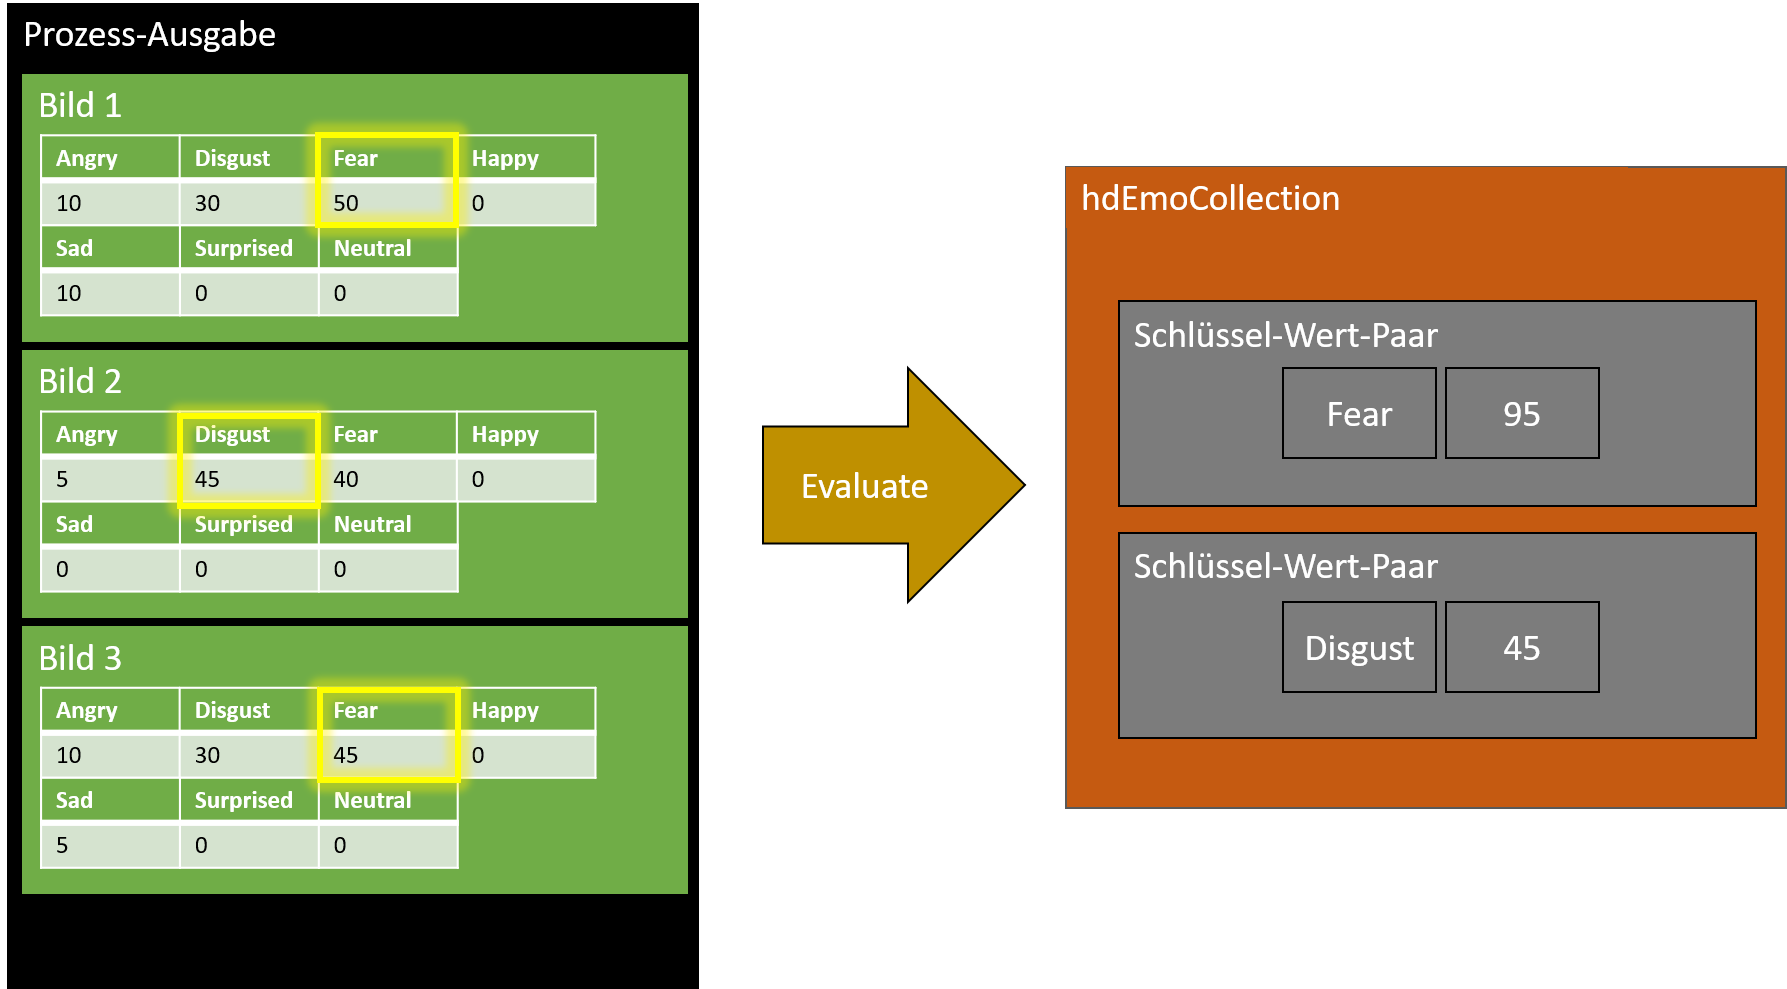
\includegraphics[scale=0.5]{Evaluate_Veranschaulichung.png}
 \caption{Visualisierung des Auswertungsvorgangs}
 \label{fig:VisualisierungEvaluation}
 \end{figure}
\subsection{GetEmotion}
Diese Funktion liefert das Schlüssel-Wert-Paar der \textit{hdEmoCollection}, welches den höchsten Wert und somit auch die höchste Gewichtung enthält. Tritt der Fall ein, dass die Emotion \textit{„Neutral“} und eine beliebig andere Emotion, beispielsweise \textit{„Happy“}, den gleichen und höchsten Wert aufweisen, liefert die \textit{GetEmotion}-Funktion \textit{„Happy“}. Bei \textit{„Neutral“} handelt es sich um keine vom Benutzer zu fordernde Emotion und somit rechtfertigt sich diese Sonderregelung.

%Lukas
\section{Reguläre Ausdrücke zur Erkennung der Resultate}
In der Klasse \textit{EmotionTableInterpreter} werden drei Reguläre Ausdrücke benutzt, um die Ergebnisse des Python-Skripts, die als Konsolenausgabe vorliegen, in das Programm zu importieren. Zwei dieser Ausdrücke werden zur Erkennung verwendet, der dritte löscht Steuerzeichen, die im Eingabestring möglicherweise vorhanden sind. Die \texttt{System.Text.RegularExpressions}-Bibliothek bindet die Funktionalität zur Verwendung der Regulären Ausdrücke ein.
\subsection{Begriffsdefinitionen}
\begin{itemize}
\item[-] Eingabestring: String, dessen Inhalt auf \textit{Matches} durchsucht wird.
\item[-] Match (\textit{plural: Matches}): Teilstring(s) des \textit{Eingabestrings}, der mit dem \textit{Pattern} übereinstimmt.
\item[-] Pattern: Regulärer Ausdruck
\item[-] Subpattern: Teil eines Regulären Ausdrucks, der benannt wird, um leichter auf ihn zugreifen zu können.
\end{itemize}
\subsection{Erkennungspattern für die Prozessausgabe}
Die folgenden Pattern werden zur Verarbeitung der Ausgabe genutzt. Die einzelnen Abschnitte werden im Folgenden erklärt. Die Darstellung des Patterns erfolgt in der Art und Weise, in der sie auch vom Computer verarbeitet werden. Dass heißt, das alle Variablennamen durch den Wert der Variablen ersetzt wurden.
\subsubsection{patternFaceFoundCount}
Das Pattern \texttt{(Faces found:  (?<FacesFoundCount>[0-9]*))\{1\}} hat den Zweck, die Anzahl der erkannten Gesichter in einem Bild auszulesen. Der Subpattern \texttt{((?<FacesFoundCount>[0-9]*))\{1\}} mit dem Namen \textit{FacesFoundCount} hat als Match eine Zahl aus dem Intervall $\left[0;9\right] \in \mathbb{N}$ und gibt diese bei Aufruf zurück. Dieser Wert wird verwendet, um zu entscheiden, ob die vom Modell erzeugten Daten im \textit{EmotionTableInterpreter} ausgewertet werden sollen, oder nicht. Im Abschnitt "PrepareModel - Konstruktor" findet sich eine genauere Erklärung.
\subsubsection{patternArray}
\texttt{$\left(?<SinglePicOutput>\\\left(\left(ar+ay\\\left(\\\left[\left(?<HighestEmotionIndex>\left[0-6\right]\right)\left(\left[,\right]\left[\right]*\left[0-6\right]\right)*\\\right]\left[, dtype=int\left[32|64\right]*\right]*\\\right)\left[,\right]\left[ \right]*\left(?<EmotionWeightArray>ar+ay\\\left(\\\left[\left(?<EmotionWeightArray0>\left[0-9\right]*\left[.\right]*\left[0-9\right]*\left[e\right]*\left[-|+\right]*\left[0-9\right]*\right)\left[,\right][ ]*(?<EmotionWeightArray1>[0-9]*[.]*[0-9]*[e]*[-|+]*[0-9]*)[,][ ]*(?<EmotionWeightArray2>[0-9]*[.]*[0-9]*[e]*[-|+]*[0-9]*)[,][ ]*(?<EmotionWeightArray3>[0-9]*[.]*[0-9]*[e]*[-|+]*[0-9]*)[,][ ]*(?<EmotionWeightArray4>[0-9]*[.]*[0-9]*[e]*[-|+]*[0-9]*)[,][ ]*(?<EmotionWeightArray5>[0-9]*[.]*[0-9]*[e]*[-|+]*[0-9]*)[,][ ]*(?<EmotionWeightArray6>[0-9]*[.]*[0-9]*[e]*[-|+]*[0-9]*)))$}
\subsection{Ablauf}


%Julia
\chapter{Material und Methoden}
Die Entwicklung des Emotionserkennungsspiel ist in drei Bereichen geteilt:
die graphische Benutzeroberfläche, die dahinter steckende Logik bzw. das
Neuronale Netz, das für die Emotionserkennung zuständig ist und die Schnittstelle
zwischen beiden. Im Folgenden werden die Methoden der einzelnen Bestandteile
des Programms beschrieben. 



\section{Neuronale Netze}
\label{subsec:statistical-summaries}
Auf Grund seiner höheren Geschwindigkeit und großen Anzahl von verschiedenen
bereitgestellten Bibliotheken gilt Python als eine der besten Programmiersprachen
für die Entwicklung einer Künstlichen Intelligenz-basierten Software.
\newline
Python wird in Kombination mit dem Deep Learning Framework  \textit{TensorFlow} angewendet, um das Netz "lehren" und seine Ergebnisse interpretieren zu können.
Bei diesem Projekt wurden die Python Version 3.6 und die TensorFlow Version
1.7 verwendet.
 \newline
Als Vorlage diente ein Beispielskript \cite{LeweOhlsenGit}, das ein Videosignal über die Webkamera
empfängt, das Video dann in einzelne Bilder (Frames) zerteilt und jedes Bild
nach Emotionen untersucht. Das Skript wurde während des Laborpraktikums
umgebaut und an die Benutzeroberfläche und die Schnittstellen angepasst.\newline
Um die einzelne Bilder zu bewerten reicht das neuronale Netz allein nicht aus. Man
benötigt auch ein Framework, das Bildverarbeitungs-Algorithmen zur Verfügung
stellt. Ein solches Framework ist OpenCV, da es sich gut mit Python kompilieren lässt.
Das ausgewählte Framework ist OpenCV in der Version ist 3.4.
 \newline
Zur Verfügung standen drei bereits trainierten neuronalen Netze bzw. Modelle: \newline
\begin{itemize}
\item[-]  FER2013 \cite{IasGoodefellow}
\item[-] CK+
\item[-] FERPlus \newline
\end{itemize}
 

Eines dieser Modelle  bindet man in das Skript ein, um auf der Basis des ausgewählten Modells die Emotionserkennung zu ermöglichen. Bei dem im Emotionserkennungsspiel verwendeten Datensatz 
handelt es sich um den FERPlus-Datensatz. 
 \cite{LeweOhlsen} Der Datensatz wurde
von einer Forschungsgruppe bei Microsoft entwickelt. Er unterscheidet sich
von seinem Vorgänger FER2013 im genaueren Crowdsourcing für den Tagging-
Vorgang.
 \cite{RamakrishnanPandeyKarmakarSaha} 
Dieser Datensatz verfügt über sieben Emotionsklassen: Wut, Ekel,
Angst, Freude, Trauer, Überraschung und neutrale Emotion.\newline
Im Gegensatz zum Beispielsskript, empfängt das für das Spiel entwickelte Skript 
keinen Stream von der Webkamera, sondern bekommt von der Benutzeroberfläche
ein Ordnerverzeichnis übergeben. In dem Ordner befinden sich Bilder, die bereits
aus dem Videostream ausgeschnitten worden sind. 
%Die Bilder werden nach der Erkennung gelöscht. Dieser Satz ist in der aktuellen Programmlogik nicht mehr gültig.
In einem Ordner sollen Bilder mit der gleichen Emotion abgespeichert werden. Die Bilder nacheinander werde
eingelesen.
 \newpage 
Zunächst wird überprüft, ob auf dem Bild ein Gesicht gefunden bzw.
erkannt werden kann. Laut den Spielregeln darf es nur einen Spieler geben,
daher liefert das Skript eine bestimmte Meldung zurück, sollte die Neuronale Netz mehr als ein Gesicht oder kein
Gesicht erkennen. Falls aber
tatsächlich ein Gesicht erkannt wird, geht das Spiel weiter. Das Gesicht auf
jedem Bild wird nach Emotionen Untersucht. Das Ergebnis wird auf der Kommandozeile
in Form eines Feldes ausgegeben, in dem auf der ersten Position das
Index von der Emotion steht, die am wahrscheinlichsten erkannt wurde.






\bibliographystyle{plain}
\bibliography{Doku}
%
\end{document}